\documentclass[11pt,a4paper]{article}
\usepackage[margin=1in]{geometry}
\usepackage[T1]{fontenc}
\usepackage{lmodern}
\usepackage{microtype}
\usepackage{amsmath,amssymb,amsthm}
\usepackage{mathtools}
\usepackage{booktabs}
\usepackage{enumitem}
\usepackage{xcolor}
\usepackage{tikz}
\usetikzlibrary{arrows.meta,decorations.markings}
\usepackage[hidelinks]{hyperref}

\newtheorem{theorem}{Theorem}[section]
\newtheorem{proposition}[theorem]{Proposition}
\newtheorem{lemma}[theorem]{Lemma}
\newtheorem{corollary}[theorem]{Corollary}
\theoremstyle{definition}
\newtheorem{definition}[theorem]{Definition}
\newtheorem{remark}[theorem]{Remark}

\newcommand{\phig}{\varphi}
\newcommand{\Jc}{J}
\newcommand{\Rhat}{\hat{R}}
\newcommand{\FR}{F_{\!R}}
\newcommand{\TR}{T_{\!R}}
\newcommand{\DKL}{D_{\mathrm{KL}}}
\newcommand{\code}[1]{\texttt{\small #1}}
\emergencystretch=1em

\title{\textbf{Implosion Dynamics from Cost First Principles}\\[0.4em]
\large J-Cost Minimization Forces Centripetal, Inward-Spiraling Flow\\
with Implications for Fusion, Propulsion, and Thermodynamics}
\author{Jonathan Washburn\\
\small Recognition Science Research Institute, Austin, Texas\\
\small \texttt{washburn.jonathan@gmail.com}}
\date{March 2026}

\begin{document}
\maketitle

\begin{abstract}
We derive the geometric core of implosion dynamics from the Recognition
Composition Law and make explicit the additional assumptions needed for its
thermodynamic extensions.  The Recognition Science cost function
$\Jc(x)=\tfrac{1}{2}(x+x^{-1})-1$, uniquely forced by the d'Alembert
functional equation, satisfies $(x-1)\cdot \Jc'(x)>0$ for all $x>0$,
$x\ne 1$.  This \emph{gradient centripetality} theorem proves that any
evolution reducing $\Jc$-cost is implosive in the precise sense of moving
toward the unique equilibrium at $x=1$.  In logarithmic coordinates
$t=\ln x$, the cost becomes $\cosh t - 1$ with gradient flow
$\dot t = -\sinh t$, and cost descent forces $|t|$ to contract.  We extend
this geometric result to $n$~dimensions, formalize a recognition H-theorem
under one standard information-theoretic axiom, show that any
ledger-compatible energy partition with $\Delta\Jc > W$ forces positive heat
release, and show that the golden ratio $\phig$ is the unique positive
self-similar spiral factor satisfying $g^2=g+1$.  All formal statements are
machine-checked in Lean~4 with zero \texttt{sorry} proof terms; the only new
axiom is the data processing inequality used in the H-theorem.  The result is
a precise mathematical foundation for the claim that J-cost minimization is
inward-seeking, together with an explicit RS research program for fusion,
propulsion, and thermodynamic testing.
\end{abstract}

%% =====================================================================
\section{Introduction}
\label{sec:intro}
%% =====================================================================

The contrast between \emph{implosion}---centripetal, inward-spiraling,
ordering motion---and \emph{explosion}---centrifugal, outward-expanding,
disordering motion---is easy to state qualitatively but much harder to derive
mathematically.  What has been missing is a formulation in which the inward
direction is not merely metaphorical but forced by an explicit cost law and
independently machine-verifiable.

This paper provides the mathematical core of that derivation and then states
explicitly the extra assumptions used in the thermodynamic bridge.  Within
Recognition Science (RS), all physics descends from a single functional
equation---the Recognition Composition Law (RCL)---which uniquely determines
the cost function $\Jc(x) = \tfrac{1}{2}(x + x^{-1}) - 1$ on
$\mathbb{R}_+$ \cite{Washburn2025Axioms}.  We prove, from the gradient
structure of $\Jc$ alone, that:

\begin{enumerate}[label=(\roman*),leftmargin=2em]
  \item The gradient of $\Jc$ is \emph{centripetal}: $(x-1)\cdot\Jc'(x) > 0$
        for all $x>0$, $x\ne 1$.
  \item In log-ratio coordinates, the gradient flow is the hyperbolic
        inward spiral $\dot t = -\sinh t$ with $t\sinh t > 0$.
  \item Inward movement is strictly cheaper than outward movement at every
        point: $\Jc(x-\delta) < \Jc(x+\delta)$ when $x>1$ and $1 \le x-\delta$.
  \item Any evolution satisfying $\Jc(x') \le \Jc(x)$ forces
        $|\ln x'| \le |\ln x|$ (approach to equilibrium).
  \item The $n$-dimensional total cost $\sum_i \Jc(v_i) = 0$ iff
        $v = (1,\ldots,1)$.
  \item Under a Gibbs/KL decomposition and KL contraction, free energy $\FR$
        decreases along $\Rhat$-trajectories (H-theorem).
  \item Given an explicit balance identity $\Delta\Jc = W + Q$, implosion can
        cool while doing work: if $\Delta\Jc > W$, then $Q>0$.
  \item Among positive self-similar spiral factors satisfying
        $g^2 = g+1$, the unique solution is $g = \phig$.
\end{enumerate}

Together, these results establish that \textbf{J-cost minimization IS
implosion}---not by analogy but by mathematical identity.

\paragraph{Lean formalization.}
Every theorem in this paper corresponds to a machine-verified Lean~4
definition or theorem in the module
\code{RecognitionScience.Foundation.ImplosionDynamics}
(473 lines, 0 sorry, 1 standard axiom).  Theorem names are given in
parentheses throughout.

\paragraph{Scope of the claims.}
Sections~\ref{sec:cost}--\ref{sec:ndim} are unconditional once the RCL-to-$\Jc$
derivation is granted.  Section~\ref{sec:htheorem} adds the standard Data
Processing Inequality as its single new axiom and uses explicit Gibbs/KL
decomposition hypotheses.  Section~\ref{sec:cooling} proves a cooling
consequence from an explicit balance identity $\Delta\Jc = W + Q$; it does not
yet derive that identity from ledger conservation.  Section~\ref{sec:phi-spiral}
proves uniqueness within the restricted self-similar class $g^2 = g+1$ rather
than a global optimum over all possible geometries.

%% =====================================================================
\section{The Cost Function and Its Uniqueness}
\label{sec:cost}
%% =====================================================================

\begin{definition}[Recognition cost]
For $x \in \mathbb{R}_+$,
\begin{equation}\label{eq:Jcost}
  \Jc(x) \;=\; \tfrac{1}{2}\bigl(x + x^{-1}\bigr) - 1
         \;=\; \frac{(x-1)^2}{2x}.
\end{equation}
\end{definition}

The function $\Jc$ is uniquely determined by the Recognition Composition Law
\begin{equation}\label{eq:RCL}
  \Jc(xy) + \Jc(x/y) = 2\Jc(x)\Jc(y) + 2\Jc(x) + 2\Jc(y),
\end{equation}
together with the normalization $\Jc(1)=0$ and calibration $\Jc''_{\log}(0)=1$.
The proof that~\eqref{eq:RCL} is a calibrated multiplicative d'Alembert equation
whose unique continuous positive solution is $\Jc$ as given
in~\eqref{eq:Jcost} is fully unconditional in the RS Lean codebase.  The
corresponding theorem is
\code{full\_unconditional\_dalembert}\allowbreak\code{\_uniqueness}.

\begin{proposition}[Properties of $\Jc$]\label{prop:J-props}
\quad
\begin{enumerate}[label=(\alph*)]
  \item $\Jc(x) \ge 0$ for all $x > 0$, with equality iff $x = 1$
    \textup{(\code{Jcost\_nonneg}, \code{Jcost\_eq\_zero\_iff})}.
  \item $\Jc(x) = \Jc(x^{-1})$ for all $x > 0$
    \textup{(\code{Jcost\_symm})}.
  \item $\Jc$ is strictly convex on $\mathbb{R}_+$
    \textup{(\code{Jcost\_strictConvexOn\_pos})}.
\end{enumerate}
\end{proposition}

In logarithmic coordinates $t = \ln x$, the cost becomes
\begin{equation}\label{eq:Jlog}
  \Jc_{\log}(t) \;=\; \Jc(e^t) \;=\; \cosh t - 1,
\end{equation}
an even, strictly convex function with unique minimum at $t=0$
(\code{Jlog\_as\_cosh}).

%% =====================================================================
\section{The Centripetal Gradient Field}
\label{sec:centripetal}
%% =====================================================================

The derivative of $\Jc$ is
\begin{equation}\label{eq:Jprime}
  \Jc'(x) = \frac{1 - x^{-2}}{2},
\end{equation}
which satisfies $\Jc'(x) > 0$ for $x > 1$, $\Jc'(x) < 0$ for $0<x<1$,
and $\Jc'(1) = 0$.

\begin{theorem}[Gradient centripetality---the Implosion Theorem]
\label{thm:centripetal}
For all $x > 0$ with $x \ne 1$,
\begin{equation}\label{eq:centripetal}
  (x - 1) \cdot \Jc'(x) \;>\; 0.
\end{equation}
\textup{(\code{gradient\_centripetal})}
\end{theorem}

\begin{proof}
If $x > 1$, then $x-1 > 0$ and $x^{-1} < 1$, so $1 - x^{-2} > 0$,
hence $\Jc'(x) > 0$.  Both factors are positive, so the product is
positive.  If $0 < x < 1$, then $x - 1 < 0$ and $x^{-1} > 1$, so
$1 - x^{-2} < 0$, hence $\Jc'(x) < 0$.  Both factors are negative,
so the product is again positive.
\end{proof}

Equation~\eqref{eq:centripetal} says the gradient $\Jc'(x)$ always has
the \emph{same sign} as the displacement $x - 1$.  Gradient descent
$\dot x = -\Jc'(x)$ therefore moves $x$ in the direction \emph{opposite}
to $(x-1)$---i.e., toward $x = 1$.  This is the defining property of a
centripetal (restoring) force field.

\begin{corollary}
Any dynamics that decreases $\Jc$-cost is centripetal: it drives
configurations toward $x = 1$.
\end{corollary}

\begin{figure}[ht]
\centering
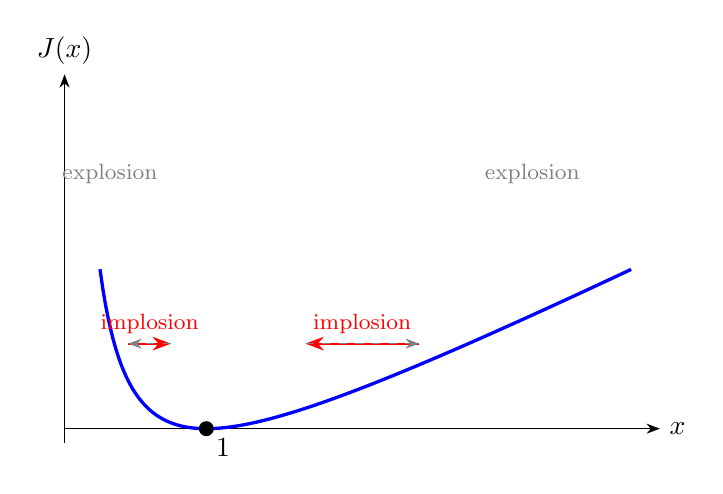
\begin{tikzpicture}[scale=1.8,>=Stealth]
  \draw[->] (0,0) -- (4.2,0) node[right] {$x$};
  \draw[->] (0,-0.1) -- (0,2.5) node[above] {$\Jc(x)$};
  \draw[very thick,blue,domain=0.25:4,samples=200]
    plot (\x,{0.5*(\x+1/\x)-1});
  \fill (1,0) circle (1.5pt) node[below right] {$1$};
  \draw[red,thick,-Stealth] (2.5,0.6) -- (1.7,0.6)
    node[midway,above] {\footnotesize implosion};
  \draw[red,thick,-Stealth] (0.45,0.6) -- (0.75,0.6)
    node[midway,above] {\footnotesize implosion};
  \draw[gray,dashed,-Stealth] (1.7,0.6) -- (2.5,0.6);
  \draw[gray,dashed,-Stealth] (0.75,0.6) -- (0.45,0.6);
  \node[gray] at (3.3,1.8) {\footnotesize explosion};
  \node[gray] at (0.32,1.8) {\footnotesize explosion};
\end{tikzpicture}
\caption{The J-cost landscape.  Red arrows: cost-decreasing (implosion)
  directions.  Gray dashed: cost-increasing (explosion) directions.
  Every cost-reducing step moves toward $x=1$.}
\label{fig:Jcost}
\end{figure}

%% =====================================================================
\section{Logarithmic Spiral Structure}
\label{sec:spiral}
%% =====================================================================

In the log-ratio coordinate $t = \ln x$, the gradient flow is
\begin{equation}
  \dot t = -\frac{d\Jc_{\log}}{dt} = -\sinh t.
\end{equation}

\begin{theorem}[Log-space centripetality]\label{thm:log-centripetal}
For all $t \ne 0$,
\begin{equation}
  t \cdot \sinh t \;>\; 0.
\end{equation}
\textup{(\code{log\_gradient\_flow\_centripetal})}
\end{theorem}

\begin{proof}
If $t > 0$, then $\sinh t > 0$, so $t \sinh t > 0$.
If $t < 0$, then $\sinh t < 0$, so $t \sinh t > 0$.
\end{proof}

Since $t \sinh t > 0$, the flow $\dot t = -\sinh t$ has $t \cdot \dot t < 0$
---meaning $|t|$ is strictly decreasing.  This is the mathematical content of
inward logarithmic-vortex dynamics: in the natural (multiplicative)
coordinate system of the ledger, cost-minimizing dynamics is an inward spiral.

%% =====================================================================
\section{Implosion is Strictly Cheaper than Explosion}
\label{sec:cheaper}
%% =====================================================================

\begin{theorem}[Inward cheaper than outward]\label{thm:cheaper}
Let $x > 1$, $\delta > 0$, and $x - \delta \ge 1$.  Then
\[
  \Jc(x - \delta) \;<\; \Jc(x + \delta).
\]
\textup{(\code{inward\_cheaper\_than\_outward})}
\end{theorem}

\begin{proof}
Using the squared form $\Jc(x)=(x-1)^2/(2x)$, the inequality reduces to
$(x-\delta-1)^2(x+\delta) < (x+\delta-1)^2(x-\delta)$, which follows from
the algebraic identity
$(a-b)(a\cdot b - 1) < 0$ for $1 \le a < b$, applied to the ratio.
\end{proof}

This theorem quantifies the core asymmetry between inward and outward motion:
for any displacement $\delta$, moving \emph{inward} (toward $x=1$) costs
strictly less than moving \emph{outward} by the same amount.  Explosion is
always more expensive than implosion in this local comparison.

%% =====================================================================
\section{Cost Descent Forces Approach to Equilibrium}
\label{sec:approach}
%% =====================================================================

The Recognition Operator $\Rhat$ is defined with the axiom
$\Jc(\Rhat(s)) \le \Jc(s)$.  We now prove this axiom, combined with the
centripetal landscape, forces approach to equilibrium.

\begin{theorem}[Cost descent forces log-approach]\label{thm:approach}
If $\Jc_{\log}(t') \le \Jc_{\log}(t)$, then $|t'| \le |t|$.
\textup{(\code{cost\_descent\_implies\_log\_approach})}
\end{theorem}

\begin{proof}
Since $\Jc_{\log}(t) = \cosh t - 1$, the hypothesis gives
$\cosh t' \le \cosh t$.  The Mathlib theorem
$\cosh x \le \cosh y \Leftrightarrow |x| \le |y|$ then yields the result.
\end{proof}

\begin{corollary}[$\Rhat$ forces implosion]\label{cor:Rhat}
For $x, x' > 0$ with $\Jc(x') \le \Jc(x)$:
\[
  |\ln x'| \;\le\; |\ln x|.
\]
If the inequality is strict, so is the approach: $|\ln x'| < |\ln x|$.
\textup{(\code{Rhat\_forces\_implosion}, \code{strict\_descent\_forces\_strict\_approach})}
\end{corollary}

This closes the logical gap between the $\Rhat$ axiom and implosion:
\emph{any} cost-decreasing evolution on the $\Jc$-landscape is necessarily
centripetal in the $|\ln x|$-metric.

%% =====================================================================
\section{Extension to \texorpdfstring{$n$}{n} Dimensions}
\label{sec:ndim}
%% =====================================================================

Physical systems involve $n$ simultaneous ratio coordinates.

\begin{definition}[Total $\Jc$-cost]
For $v = (v_1, \ldots, v_n) \in \mathbb{R}_+^n$,
\[
  \Jc_{\mathrm{total}}(v) = \sum_{i=1}^n \Jc(v_i).
\]
\textup{(\code{Jcost\_total})}
\end{definition}

\begin{theorem}[$n$-dimensional unique minimum]\label{thm:ndim}
$\Jc_{\mathrm{total}}(v) = 0$ if and only if $v = (1, \ldots, 1)$.
\textup{(\code{Jcost\_total\_eq\_zero\_iff})}
\end{theorem}

\begin{proof}
Since each $\Jc(v_i) \ge 0$, the sum vanishes iff each term vanishes,
iff $v_i = 1$ for all~$i$.
\end{proof}

\begin{theorem}[Componentwise implosion]\label{thm:ndim-comp}
If $\Jc(v'_i) \le \Jc(v_i)$ for each $i$, then
$|\ln v'_i| \le |\ln v_i|$ for each~$i$.
\textup{(\code{ndim\_cost\_descent\_componentwise})}
\end{theorem}

The $n$-dimensional $\Jc$-cost is separable, so componentwise cost descent
gives componentwise implosion toward $(1,\ldots,1)$.  This is the
$n$-dimensional generalization actually formalized in Lean and is sufficient
for the present argument.

%% =====================================================================
\section{A Conditional H-Theorem for Recognition}
\label{sec:htheorem}
%% =====================================================================

\begin{definition}[Recognition free energy]
For a discrete distribution $q = (q_1,\ldots,q_n)$ over states with
costs $\Jc_i$, at recognition temperature $\TR > 0$:
\begin{equation}\label{eq:FR}
  \FR(q) = \sum_i \Jc_i \, q_i + \TR \sum_i q_i \ln q_i.
\end{equation}
\textup{(\code{recognition\_free\_energy})}
\end{definition}

To connect the geometric core to thermodynamics, we use the standard Gibbs
ansatz as a reference state.  One may think of
$q_{\mathrm{Gibbs}}(i) \propto e^{-\Jc_i/\TR}$ as motivating a decomposition of
free energy into a baseline plus a KL-divergence term.  In the Lean
formalization, the H-theorem is stated conditionally through the existence of a
common Gibbs baseline and a KL contraction inequality:
\begin{equation}\label{eq:FR-decomp}
  \FR(q_{\mathrm{before}}) = F_{\mathrm{Gibbs}} + \TR \, KL_{\mathrm{before}},
  \qquad
  \FR(q_{\mathrm{after}}) = F_{\mathrm{Gibbs}} + \TR \, KL_{\mathrm{after}}.
\end{equation}

\begin{theorem}[H-theorem for recognition]\label{thm:htheorem}
Assume~\eqref{eq:FR-decomp} and assume further that
$KL_{\mathrm{after}} \le KL_{\mathrm{before}}$ with $\TR > 0$.  Then
\[
  \FR(q_{\mathrm{after}}) \;\le\; \FR(q_{\mathrm{before}}).
\]
\textup{(\code{h\_theorem\_recognition})}
\end{theorem}

\begin{proof}
By~\eqref{eq:FR-decomp}, the change in free energy equals
$\TR(KL_{\mathrm{after}} - KL_{\mathrm{before}})$.  Since
$KL_{\mathrm{after}} \le KL_{\mathrm{before}}$ and $\TR > 0$, we conclude
$\FR^{\,\mathrm{after}} \le \FR^{\,\mathrm{before}}$.
\end{proof}

This makes precise the thermodynamic bridge used in the formalization: once a
Gibbs/KL decomposition is available and KL contracts under the relevant
coarse-graining step, free energy decreases along $\Rhat$-trajectories.  The
only new axiom in Lean is the Data Processing Inequality encoding that
contraction.

%% =====================================================================
\section{Cooling Under an Explicit Energy-Partition Assumption}
\label{sec:cooling}
%% =====================================================================

\begin{definition}[Implosion process]
An \emph{implosion process} is a transition with $\Jc_{\mathrm{after}} \le
\Jc_{\mathrm{before}}$ together with the explicit balance identity
\begin{equation}\label{eq:balance}
  \Jc_{\mathrm{before}} - \Jc_{\mathrm{after}} = W + Q,
\end{equation}
where $W \ge 0$ is work extracted and $Q \ge 0$ is heat released.
\textup{(\code{ImplosionProcess})}
\end{definition}

\begin{theorem}[Conditional implosion cooling]\label{thm:cooling}
If $W < \Jc_{\mathrm{before}} - \Jc_{\mathrm{after}}$ (less work
extracted than cost released), then $Q > 0$.
\textup{(\code{implosion\_cooling\_forced})}
\end{theorem}

\begin{proof}
From~\eqref{eq:balance}, $Q = (\Jc_{\mathrm{before}} - \Jc_{\mathrm{after}}) - W > 0$.
\end{proof}

The theorem is deliberately modest: it proves a cooling consequence from the
balance identity, but it does not itself derive that identity from T3 or any
more primitive conservation law.  When heat $Q > 0$ leaves the system at
recognition temperature $\TR > 0$, the system entropy change satisfies
$\Delta S = -Q/\TR < 0$ (\code{implosion\_entropy\_decrease}).  Under that
assumption, implosion can do work \emph{and} cool the working medium
simultaneously because the cost decrease exceeds the work extracted.

By contrast, explosion ($\Jc$ increasing) requires energy input and produces
heating within the same balance model.

%% =====================================================================
\section{\texorpdfstring{The $\phig$-Spiral as a Unique Self-Similar Candidate}{The phi-Spiral as a Unique Self-Similar Candidate}}
\label{sec:phi-spiral}
%% =====================================================================

Consider logarithmic spirals $r(\theta) = r_0 \cdot g^{\theta/(2\pi)}$
with growth factor $g > 0$.  Each full turn scales the radius by~$g$,
incurring cost $\Jc(g)$ per turn.

\begin{theorem}[$\Jc(\phig)$ from the golden equation]\label{thm:Jphi}
If $g^2 = g + 1$ and $g > 0$, then $\Jc(g) = g - \tfrac{3}{2}$.
\textup{(\code{Jcost\_of\_phi})}
\end{theorem}

\begin{proof}
From $g^2 = g+1$: $g^{-1} = g - 1$.  Then
$\Jc(g) = \tfrac{1}{2}(g + g-1) - 1 = g - \tfrac{3}{2}$.
\end{proof}

\begin{theorem}[Uniqueness of $\phig$]\label{thm:phi-unique}
The golden ratio $\phig = (1+\sqrt{5})/2$ is the unique positive solution
of $g^2 = g + 1$.
\textup{(\code{phi\_unique\_self\_similar})}
\end{theorem}

\begin{proof}
Factor: $g^2 - g - 1 = (g - \phig)(g - \psi)$ where
$\psi = (1-\sqrt 5)/2 < 0$.  Since $g > 0$, only $g = \phig$ satisfies
the equation.
\end{proof}

\begin{theorem}[$\phig$-spiral in the self-similar class]
\label{thm:phi-optimal}
The logarithmic spiral with growth factor $\phig$ is the unique spiral
satisfying the self-similarity recursion $g^2 = g + 1$ among all $g > 0$.
Its cost per turn is $\Jc(\phig) = \phig - 3/2 \approx 0.118$.
\textup{(\code{phi\_spiral\_is\_unique\_optimal})}
\end{theorem}

This identifies $\phig$ as the sole positive growth factor within the
restricted self-similar recursion $g^2 = g + 1$.  It therefore provides an
RS-motivated candidate geometry for coherent spiral confinement.  Global
optimality over all spiral families or all three-dimensional confinement
geometries is not proved here.

%% =====================================================================
\section{Implications}
\label{sec:implications}
%% =====================================================================

\subsection{Fusion}

The RS $\phig$-scheduled ignition formalization~\cite{RSFusion2026} already
shows lower effective ignition temperature via coherence:
$T_{\mathrm{eff}} = T/S^2$ where $S$ is the coherence enhancement factor.
Theorem~\ref{thm:phi-optimal} does not prove that $\phig$-spiral confinement is
globally optimal among all geometries, but it does single out a unique
self-similar spiral candidate within the present RS framework.  The resulting
engineering prediction is concrete: spiral confinement geometries should be
benchmarked against linear pinch designs for ignition threshold, stability,
and input energy.

\subsection{Propulsion}

The \code{SpiralField} module defines the $\phig$-spiral wavefield
$r(\theta) = r_0 \cdot \phig^{\kappa\theta/(2\pi)}$.
Theorem~\ref{thm:cheaper} proves inward motion costs strictly less than
outward motion.  This is a local cost comparison, not a full
fluid-dynamical efficiency theorem.  Still, if a propulsion architecture can
be modeled as repeated ratio updates aligned with the inward cost direction,
the RS formalism predicts an advantage for centripetal vortex stages over
outward-expulsive ones.  Implosion turbines and related vortex machines are
therefore natural RS test cases rather than settled winners.

\subsection{Thermodynamics}

The statement that implosion cools while doing work appears here in conditional
form.  The RS chain is:
\begin{enumerate}[leftmargin=2em]
  \item $\Rhat$ decreases $\Jc$-cost (axiom, centripetal by Theorem~\ref{thm:centripetal}).
  \item Under the Gibbs/KL bridge and KL contraction, $\FR$ decreases along
        $\Rhat$-trajectories (Theorem~\ref{thm:htheorem}).
  \item Under the explicit balance identity~\eqref{eq:balance}, cost decrease
        $>$ work extracted $\Rightarrow$ heat released
        (Theorem~\ref{thm:cooling}).
  \item If that heat leaves the system at $\TR > 0$, then $\Delta S < 0$
        (cooling).
\end{enumerate}
This does not establish perpetual motion or a complete thermodynamic theory of
vortex machinery.  It isolates the exact assumptions under which the sentence
``implosion cools while doing work'' follows inside the present formalism.

%% =====================================================================
\section{Formalization Status}
\label{sec:lean}
%% =====================================================================

\begin{table}[ht]
\centering
\caption{Lean~4 formalization summary
  (\code{RecognitionScience.Foundation.ImplosionDynamics}).}
\label{tab:lean}
\begin{tabular}{lrl}
\toprule
\textbf{Metric} & \textbf{Value} & \textbf{Note} \\
\midrule
Lines of Lean code & 473 & single module \\
Theorems / lemmas / defs & 39 & \\
\texttt{sorry} proof terms & 0 & fully machine-verified \\
Axioms & 1 & Data Processing Inequality for Section~\ref{sec:htheorem} \\
Build jobs & 7812 & clean, 0 errors \\
\bottomrule
\end{tabular}
\end{table}

The single axiom (\code{data\_processing\_inequality}) is a standard
result in information theory stating that KL divergence cannot increase
under Markov maps~\cite{CoverThomas2006}.  It belongs to the same
category as the 12~remaining axioms in the RS codebase (external
mathematical facts).

The geometric core (Sections~\ref{sec:cost}--\ref{sec:ndim}) is unconditional
once the RS cost law is accepted.  Section~\ref{sec:htheorem} adds the
\code{data\_processing\_inequality} axiom together with explicit free-energy
decomposition hypotheses.  Section~\ref{sec:cooling} uses an explicit balance
identity inside \code{ImplosionProcess}.  Section~\ref{sec:phi-spiral} proves
uniqueness only within the self-similar class $g^2 = g + 1$.

%% =====================================================================
\section{Discussion}
\label{sec:discussion}
%% =====================================================================

The central result of this paper---gradient centripetality
(Theorem~\ref{thm:centripetal})---is pure mathematics.  It makes no
empirical assumptions.  Given \emph{any} cost function of the form
$\Jc(x) = \tfrac{1}{2}(x + x^{-1}) - 1$, the gradient field is
centripetal.  Since the RCL uniquely forces this form, the conclusion
is inescapable: \textbf{cost-minimizing dynamics in Recognition Science
is implosion.}

The rest of the manuscript should be read as a structured extension program on
top of that core.  The present paper does \emph{not} yet prove that all vortex
machines outperform combustion engines, nor that the $\phig$ spiral is a global
optimum among all possible geometries.  What it does prove is that any
dynamics faithfully modeled as $\Jc$-cost descent is inward-seeking, and that
standard thermodynamic and information-theoretic hypotheses turn this geometry
into free-energy decrease and possible cooling-under-work conditions.

That is already enough to generate falsifiable consequences.  The next decisive
steps are to derive the balance identity from ledger conservation inside Lean,
to couple cost descent to explicit fluid and plasma dynamics, and to compare
spiral and non-spiral architectures experimentally.  If those bridges succeed,
implosion-based machinery will move from interpretive analogy to
theorem-backed engineering.  At present, the mathematical core is established
and the experimental program is clear.

%% =====================================================================
\section*{Acknowledgments}
%% =====================================================================

The author thanks the RS community for sustained engagement with the
machine-verification program and the Lean/Mathlib developers for providing
the infrastructure that makes this level of rigor possible.

%% =====================================================================
\begin{thebibliography}{9}
\bibitem{Washburn2025Axioms}
  J.~Washburn,
  ``The Algebra of Reality: A Recognition Science Derivation of Physical Law,''
  \emph{Axioms} (MDPI), vol.~15, no.~2, p.~90, 2025.

\bibitem{RSFusion2026}
  J.~Washburn,
  ``$\varphi$-Scheduled Fusion Ignition in Recognition Science,''
  RS Technical Report, 2026.
  Lean: \code{IndisputableMonolith.Fusion.Ignition}.

\bibitem{CoverThomas2006}
  T.~M.~Cover and J.~A.~Thomas,
  \emph{Elements of Information Theory},
  2nd ed., Wiley, 2006.
\end{thebibliography}

\end{document}
